%%%%%%%%%%%%%%%%%%%%%%%%%%%%%%%%%%%%%%%%%%%%%%%%%%%%%%%%%%%%%%%%%%%%
%%\documentclass[master]{hdu-thesis}[]中不同的模式选择对应不同的模板%%%%
%|master| 学术型硕士学位论文模板 |
%|promaster| 专业学位硕士学位论文模板 |
%|master_review| 学术型硕士送审模板 |
%|promaster_review| 专业学位硕士送审模板 |
%%%%%%%%%%%%%%%%%%%%%%%%%%%%%%%%%%%%%%%%%%%%%%%%%%%%%%%%%%%%%%%%%%%%%%
\documentclass[master]{hdu-thesis}
% \documentclass[master_review]{hdu-thesis}
% \documentclass[promaster]{hdu-thesis}
% \documentclass[promaster_review]{hdu-thesis}

\title{学位论文中文题目}{Thesis Title in English}%%%%%%论文标题，前者对应中文标题，后者对应英文标题
\author{姓名}{Name}%%%%%%作者
\advisor{姓名~教授}{Prof. Name}%%%%%%指导老师
% \secondadvisor{导师姓名~职称}{Prof. Name}%%%%%%第二指导老师，没有一定要注释，大部分人没有第二指导老师，忽略这个命令即可
\school{自动化学院}{School of Automation}%%%%学院
\major{控制科学与工程}{Control Science and Engineering}%%%%%%%%%%专业
\majorfield{专业领域中文名}{Major Field in English}%%%%%%专业领域（仅专硕填写，仅promaster模式封面显示）
\authornumber{**********}%%%%%%学号
\confidential{}%%%%%%密级（仅限于论文来源于国防军工项目时填写，非国防项目请留空）
\delaypublic{否}%%%%%%是否延期公开
\schoolcode{10336}%%%%%%学校代码
\completedate{2026}{5}{May}  %%%%%%设计完成时间
\authordirection{研究方向}{Research Interests}%%%%研究方向前者对应中文方向，后者对应英文，仅盲审模式使用

\usepackage{makecell}

\begin{document}

%%%%%%%%%%%%%%%%插入封面%%%%%%%%%%%
\makecover
%%%%%%%%%%%%%%%%插入原创性声明%%%%%%%%%
\makedeclaration

%%%%%%%%%%%%%%%中文摘要%%%%%%%%%%%%%%
\cnabstract

中文摘要

\cnkeyword{关键词1，关键词2，关键词3，关键词4}

%%%%%%%%%%%%%%%英文摘要%%%%%%%%%%%%
\enabstract

English Abstract

\enkeyword{Keyword1, Keyword2, Keyword3, Keyword4}




%%%%%%%%%%%%图目录%%%%%%%%%%%%%%%%
\figurelist
%%%%%%%%%%%%%%%%%%%

% %%%%%%%%%%%%表格目录%%%%%%%%%%%%%
\tablelist

% %%%%%%%%%%%%目录%%%%%%%%%%%
\tableofcontents

% %%%%%%%%%%%%%%%%%%%%%%%%

%%%%%%%%%%%%%%%正文%%%%%%%%%%%%

\chapter{绪论}

\section{研究背景与意义}

人类大脑是自然界已知最复杂的智能系统，在感知、认知、情绪加工及行为决策等多层次任务中展现出卓越的效率与灵活性\citep{hassabis2017neuroscience}。理解大脑如何在复杂环境中处理信息、形成认知并驱动行为，是神经科学、认知科学以及人工智能领域长期关注的核心问题。随着神经科学与计算科学的协同发展，利用计算模型解析神经活动，并逆向重建其对应的认知状态或行为意图，已成为脑科学与人工智能交叉融合的重要方向\citep{haynes2006decoding}。神经信号解码作为连接生物智能与人工智能的关键桥梁\citep{wolpaw2007brain}，对于揭示大脑信息处理机制及推动新一代类脑人工智能系统发展具有重要意义\citep{makeig2012evolving}。

近年来，脑机接口（Brain–Computer Interface, BCI）\citep{gao2021interface}技术的发展进一步推动了神经信号解码研究的深入。BCI系统通过直接采集并解析大脑神经活动，实现人类与外部设备之间的直接交互，从而为运动功能障碍患者提供辅助控制能力，并拓展了人机交互的技术路径\citep{kawala2021summary,gao2025brain}。非侵入式BCI因其安全性高、成本低和易于推广等优势，在临床康复、人机交互、情绪监测等领域展现出广阔的应用前景。常见的非侵入式神经信号主要包括脑电图（Electroencephalography, EEG）\citep{al2018review}、脑磁图（Magnetoencephalography, MEG）\citep{mellinger2007meg, hajipour2012selection}、功能性近红外光谱（functional Near-Infrared Spectroscopy, fNIRS）\citep{shin2020performance, lim2020unified}以及功能性磁共振成像（functional Magnetic Resonance Imaging, fMRI）\citep{yoo2004brain, weiskopf2003physiological}等。这些神经成像技术从不同角度刻画大脑活动，为研究复杂脑功能提供了重要数据来源。然而，由于脑信号本身具有高噪声、强非线性以及显著个体差异等特点，如何从复杂的神经数据中准确、稳定地解码人类意图与认知状态，仍然是脑机接口研究领域面临的关键挑战。

\section{国内外研究现状}

\subsection{EEG单模态解码的研究现状}

EEG能够以毫秒级时间分辨率记录大脑皮层神经元群体的电活动变化，是当前非侵入式BCI研究中最常用的神经信号之一。由于其采集设备成本较低、操作相对简便，并且能够直接反映神经电活动的动态变化，EEG被广泛应用于运动想象识别、认知状态监测以及情绪识别等多种BCI任务中\citep{al2018review,sitaram2009hemodynamic}。随着BCI研究的不断发展，如何从复杂且高噪声的EEG信号中提取具有判别力的神经特征并实现可靠解码，成为该领域的重要研究问题。

通常，EEG信号解码过程可以划分为三个关键步骤：预处理、特征提取和分类，如图~\ref{fig:figure1}~所示。预处理阶段用于去除噪声与伪迹，为后续分析提供更稳定的信号基础；特征提取阶段将原始脑电信号转换为具有判别能力的紧凑表示；分类阶段则根据提取的特征识别不同的脑状态或行为意图。

\begin{figure}[htbp]
    \centering
    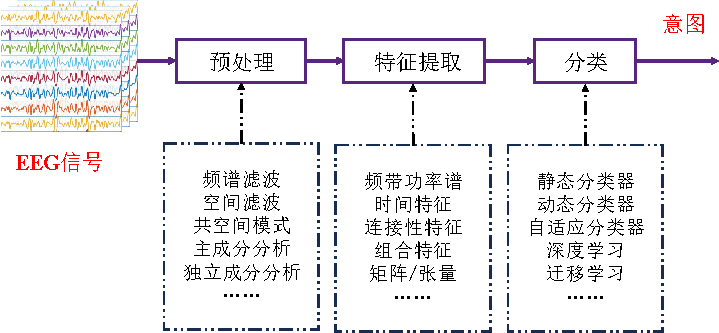
\includegraphics[scale=1]{pic/图片0-crop.pdf}
    \caption{EEG信号解码基本流程}
    \label{fig:figure1}
\end{figure}

\subsection{研究现状2}
 
\subsection{研究现状3}

\subsection{现有研究的不足与挑战}

综上所述，尽管已有研究取得了一定进展，但由于××××，现有方法仍面临以下共性挑战：

\section{研究内容与章节安排}

\subsection{研究内容}

针对现有研究的不足与挑战，本文围绕……，系统开展方法研究，构建……，整体研究思路如图~\ref{fig:figure0}~所示。具体研究内容包括：

\begin{figure}[H]
    \centering
    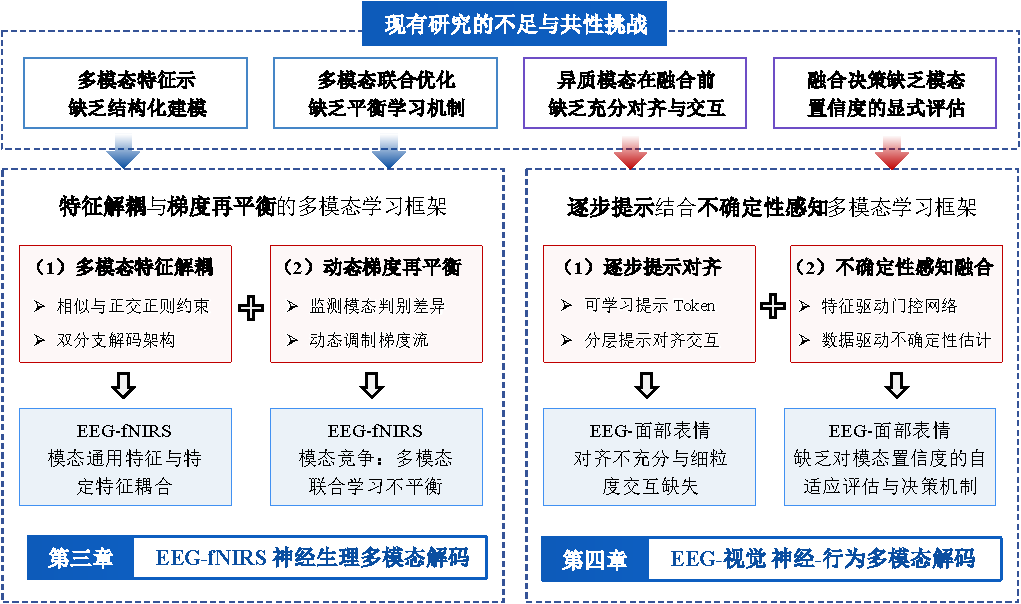
\includegraphics[scale=0.85]{pic/图片1-crop.pdf}
    \caption{本文整体研究思路}
    \label{fig:figure0}
\end{figure}

\subsection{章节安排}

本文的整体章节安排如下：

\textbf{第一章~绪论：}介绍研究背景与研究意义，……。

\textbf{第二章~×××：}系统介绍本文涉及的……相关基础理论，为后续研究提供支撑。

\textbf{第三章~×××：}……。

\textbf{第四章~×××：}……。

\textbf{第五章~总结与展望：}总结全文研究工作与主要创新成果，分析……方面的局限性，并对未来研究方向进行展望。

\chapter{第二章相关基础标题}

\section{引言}

\section{小节标题1}

\subsection{小节子标题1.1}

\subsection{小节子标题1.2}

\subsection{小节子标题1.3}

\section{小节标题2}

\subsection{小节子标题2.1}

\subsection{小节子标题2.2}

\subsection{小节子标题2.3}

\section{小节标题3}

\subsection{小节子标题3.1}

\subsection{小节子标题3.2}

\subsection{小节子标题3.3}

\subsection{小节子标题3.4}

\section{本章小结}



\chapter{第三章标题}

\section{引言}

\section{提出的方法或者框架名称}

\subsection{子标题1}

\subsection{子标题2}

\subsection{子标题3}

\subsection{子标题4}

\subsection{子标题5}

\subsection{子标题6}

\section{实验与结果分析}

\subsection{数据集介绍}

\subsection{数据预处理}

\subsection{实验细节}

\subsection{子标题4}

表~\ref{tab:tabel1.2}~和表~\ref{tab:tabel1.3}~分别汇报了详细比较结果，

\begin{table}[htb]
  \caption{xxxxx性能比较}
  \centering
  \wuhao
  % 调整列间距以美化排版
  \setlength{\tabcolsep}{6mm}{
  \renewcommand{\arraystretch}{1.5}
  \begin{tabular}{cccc}
    \toprule
    任务 & 方法 & 指标1（\%）  & 指标2（\%） \\
    \midrule
    \multirow{6}{*}{任务1} 
    & 1   & $00.00^* \pm 00.00$ & $00.00 \pm 00.00$ \\
    & 2   & $00.00^* \pm 00.00$ & $00.00 \pm 00.00$ \\
    & 3   & $00.00^* \pm 00.00$ & $00.00 \pm 00.00$ \\
    & 4   & $00.00^* \pm 00.00$ & $00.00 \pm 00.00$ \\
    & 5   & $00.00^* \pm 00.00$ & $00.00 \pm 00.00$ \\
    & 本章方法     & $\textbf{00.00} \pm 00.00$ & $\textbf{00.00} \pm 00.00$ \\
    \cmidrule{1-4}
    \multirow{6}{*}{任务2} 
    & 1   & $00.00^* \pm 00.00$ & $00.00 \pm 00.00$ \\
    & 2   & $00.00^* \pm 00.00$ & $00.00 \pm 00.00$ \\
    & 3   & $00.00^* \pm 00.00$ & $00.00 \pm 00.00$ \\
    & 4   & $00.00^* \pm 00.00$ & $00.00 \pm 00.00$ \\
    & 5   & $00.00^* \pm 00.00$ & $00.00 \pm 00.00$ \\
    & 本章方法    & $\textbf{00.00} \pm 00.00$ & $\textbf{00.00} \pm 00.00$ \\
    \cmidrule{1-4}
    \multirow{6}{*}{任务3} 
    & 1   & $00.00^* \pm 00.00$ & $00.00 \pm 00.00$ \\
    & 2   & $00.00^* \pm 00.00$ & $00.00 \pm 00.00$ \\
    & 3   & $00.00^* \pm 00.00$ & $00.00 \pm 00.00$ \\
    & 4   & $00.00^* \pm 00.00$ & $00.00 \pm 00.00$ \\
    & 5   & $00.00^* \pm 00.00$ & $00.00 \pm 00.00$ \\
    & 本章方法     & $\textbf{00.00} \pm 00.00$ & $\textbf{00.00} \pm 00.00$ \\
    \bottomrule
  \end{tabular}}
  \\ \vspace{1ex} % 表格与注脚之间留一点间距

  \vspace{-1ex} % 微调间距
  \begin{flushleft}
    \footnotesize 注：“*” 表示与本章方法相比具有显著性差异（$p < 0.01$，配对 t 检验）。
  \end{flushleft}
  \label{tab:tabel1.2}
\end{table}

\begin{table}[htb]
  \caption{xxxxx性能比较}
  \centering
  \wuhao
  % 调整列间距以美化排版
  \setlength{\tabcolsep}{6mm}{
  \renewcommand{\arraystretch}{1.5}
  \begin{tabular}{cccc}
    \toprule
    任务 & 方法 & 指标1（\%）& 指标2（\%） \\
    \midrule
    \multirow{6}{*}{任务1} 
    & 1     & $00.00^* \pm 00.00$ & $00.00 \pm 00.00$ \\
    & 2     & $00.00^* \pm 00.00$ & $00.00 \pm 00.00$ \\
    & 3     & $00.00^* \pm 00.00$ & $00.63 \pm 00.00$ \\
    & 4     & $00.00^* \pm 00.00$ & $00.00 \pm 00.00$ \\
    & 5     & $00.00^* \pm 00.00$ & $00.00 \pm 00.00$ \\
    & 本章方法     & $\textbf{00.00} \pm 00.00$ & $\textbf{00.00} \pm 00.00$ \\
    \cmidrule{1-4}
    \multirow{6}{*}{任务2} 
    & 1     & $00.00^* \pm 00.00$ & $00.00 \pm 00.00$ \\
    & 2     & $00.00^* \pm 00.00$ & $00.00 \pm 00.00$ \\
    & 3     & $00.00^* \pm 00.00$ & $00.00 \pm 00.00$ \\
    & 4     & $00.00^* \pm 00.00$ & $00.00 \pm 00.00$ \\
    & 5     & $00.00^* \pm 00.00$ & $00.00 \pm 00.00$ \\
    & 本章方法     & $\textbf{00.00} \pm 00.00$ & $\textbf{00.00} \pm 00.00$ \\
    \cmidrule{1-4}
    \multirow{6}{*}{任务3} 
    & 1    & $99.16 \pm 01.58$   & $99.16 \pm 01.58$ \\
    & 2    & $92.74^* \pm 06.41$ & $92.75 \pm 06.39$ \\
    & 3    & $96.11^* \pm 01.84$ & $96.13 \pm 01.83$ \\
    & 4    & $97.22^* \pm 01.24$ & $97.22 \pm 01.24$ \\
    & 5    & $98.33^* \pm 01.04$ & $98.33 \pm 01.04$ \\
    & 本章方法     & $\textbf{00.00} \pm 00.00$ & $\textbf{00.00} \pm 00.00$ \\
    \bottomrule
  \end{tabular}}
  \\ \vspace{1ex} % 表格与注脚之间留一点间距

  \vspace{-1ex} % 微调间距
  \begin{flushleft}
    \footnotesize 注：“*” 表示与本章方法相比具有显著性差异（$p < 0.01$，配对 t 检验）。
  \end{flushleft}
  \label{tab:tabel1.3}
\end{table}

\subsection{子标题5}

\section{讨论与分析}

\subsection{消融实验}

\subsection{子标题2}

\subsection{子标题3}

\subsection{子标题4}

\subsection{子标题5}

\subsection{局限性与未来工作}

尽管所提框架取得了有价值的实验结果，仍存在以下几方面值得深入探讨的局限性。

\section{本章小结}


 
\chapter{第四章标题}

\section{引言}

\section{提出的方法或者框架名称}

\subsection{框架概述}

\subsection{子标题2}

\subsection{子标题3}

\subsection{子标题4}

\subsection{子标题5}

\section{实验与结果分析}

\subsection{数据集与实验协议}

\subsection{子标题2}

\subsection{子标题3}

\subsection{子标题4}

\section{讨论与分析}

\subsection{子标题1}

\subsection{子标题2}

\subsection{子标题3}

\subsection{子标题4}

\subsection{子标题5}

\subsection{局限性与未来工作}

\section{本章小结}


%%%%%%%%%%%%%%%%% 总结与展望 %%%%%%%%%%%%%%%%%%
\chapter{总结与展望}

\section{工作总结}

\section{研究展望}

%%%%%%%%%%%%%%%%%致谢%%%%%%%%%%%%%%%%%%%%%%%%%%

\acknowledgement
   
谨向本研究所参考与借鉴的国内外文献与前沿成果致以诚挚的敬意。正是这些凝聚着无数研究者智慧与心血的工作，构筑了本论文得以展开的学术基础，使我能够站在前人的肩膀上，理解问题、探索问题，并尝试给出自己的回答。

感谢父母！他们从未站在高处，却倾尽所有将我举过头顶，让我能够看到他们从未见过的天空。这份恩情，写不进参考文献，却刻在我每步前行的足迹中。

一切尽在不言中，感谢所有影响过我的人！感谢自己，感谢自己所经历的一切，感谢自己一路前行！

人生路远，请永远别放弃学习！
 
% 盲审不加致谢
%%%%%%%%%%%%%%%%%%%%%%%%%%%%%%%%%%%%%%%%

%%%%%%%%%%%%%%%%%%%%%%%%%%%%%参考文献%%%%%%%%%%%%%%%%%%%%%%%%%%%%%%%%%
\hdubibliography{ref/reference}

%%%%%%%%%%%%%%%%%%%%%%%%%%%%%个人成果%%%%%%%%%%%%%%%%%%%%%%%%%%%%%%%%%
% % !Mode:: "TeX:UTF-8"

\personalresult

\begin{enumerate}
  \item  Author A, Author B, Author C, et al.\newblock xxxxx[J]. \newblock Neurocomputing, 2025, 638 : xxxxx. （导师一作，本人第二；中科院 SCI 二区，Top；对应本文第三章）
  \item Author B, Author A, Author C, et al. \newblock xxxxx[J].  \newblock IEEE Transactions on Affective Computing, 2026, 17(1): xxx – xxx. （第一作者；中科院 SCI 一区，Top；对应本文第四章）
\end{enumerate}
 %盲审不加个人成果而是全部放在附录中
% %%%%%%%%%%%%%%%%%%%%%%%%%%%%%附录%%%%%%%%%%%%%%%%%%%%%%%%%%%%%%%%%%%%

\singleappendix

{\par\bfseries \noindent 攻读硕士期间的主要成果：}
\begin{enumerate}
  \item  xxxxx. \newblock xxxxx [J].\newblock Neurocomputing, 2025, xxx: xxxxxx. （导师一作，本人第二；中科院SCI二区Top；对应本文第3章）
  \item xxxx.\newblock xxxxx [J].\newblock IEEE Transactions on Affective Computing, 2026, 17(1): xxx - xxx. （第一作者；中科院SCI一区Top；对应本文第4章）
\end{enumerate}

\end{document}
